Fuel prices significantly influence transportation choices, affecting both consumer behavior and industry trends. While the cost of traditional fuels like petroleum and diesel remains a key factor, the growing shift to electric vehicles (EVs) brings electricity prices into focus. This section examines the pricing dynamics of electricity and fossil fuels, shedding light on the economic factors that impact their costs.

Figure \ref{fig: fuel_prices} illustrates the price changes over the past 20 years. Both fuel types follow similar trends, with diesel typically being cheaper than its counterpart. As of April 7th, 2025, the prices for petroleum and diesel were \texteuro 1,785 and \texteuro1,551 per 1,000 liters, respectively.

\begin{figure}[H]
	\begin{center}
		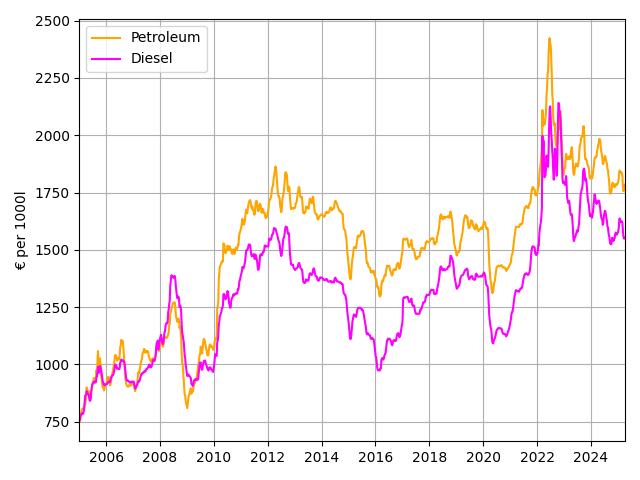
\includegraphics[width=\linewidth]{images/gas_diesel_prices.png}
		\caption{Fuel Prices throughout the Years}
		\label{fig: fuel_prices}
		\captionsetup{font={footnotesize,bf,it}}
		\caption*{Data: European Commission, \cite{PriceDevelopments}} 
	\end{center}
\end{figure}
Figure \ref{fig: electr_bill} shows the electricity bill values for consumers, divided into two categories: households and non-households. Non-household consumers, such as charging point operators and industrial users, often benefit from more favorable rates due to higher efficiency, larger volumes, and more consistent demand. The specific types of distributors are listed in the legend of Figure \ref{fig: electr_bill}. A noticeable peak in household electricity expenses occurred following the onset of the Ukraine-Russia war. For non-households, prices have shown a general upward trend over time. In 2023, the Preisbremse (price cap) was introduced to mitigate the economic impact of the energy crisis. \cite{BundesregierungStromPreisBremse}
\begin{figure}[H]
	\begin{center}
		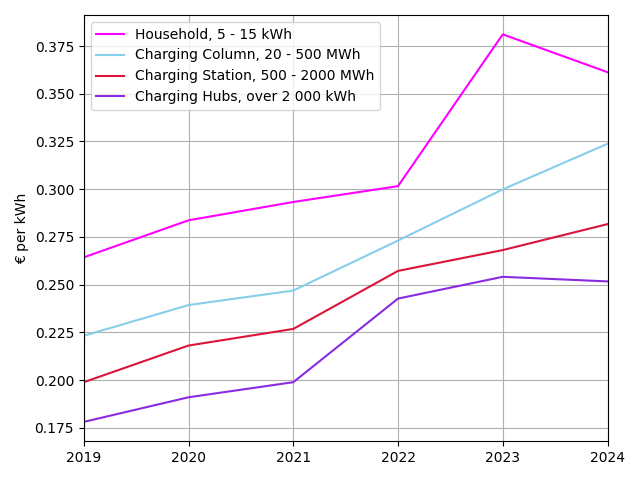
\includegraphics[width=\linewidth]{images/Elec_price.png}
	\caption{Charging Cost per kWh over the Years}
	\label{fig: electr_bill}
	\captionsetup{font={footnotesize,bf,it}}
	\caption*{Data: Statistisches Bundesamt, \cite{DestatisStrompreise}, \cite{GENESISHaushalt}, \cite{GENESISNichtHaushalt}}
	\end{center}
\end{figure}

It is important to note that the electricity bill values presented do not reflect the actual prices consumers pay when charging their electric vehicles (EVs), but rather the average electricity prices paid by households and non-household distributors for grid energy. Home charging is classified as slow charging, while a column typically refers to slow or normal public charging. A station provides fast charging, and a hub is used for ultra-fast charging, offering the quickest recharge times. Since detailed pricing data for individual distributor types was unavailable, representative values were estimated using ChatGPT: \texteuro0.49 for standard columns, \texteuro0.59 for stations, \texteuro0.69 for hubs, and \texteuro0.40 for Tesla Superchargers. A grid efficiency factor of 85\% was also applied to account for typical charging losses. Additionally, ChatGPT provided estimated vehicle data—such as tank size, battery capacity, and electric (RE) and combustion (RC) ranges by body type—which is summarized in Figure \ref{fig: vehic_data} to support the simplified cost model.
\begin{figure}[H]
	\begin{center}
		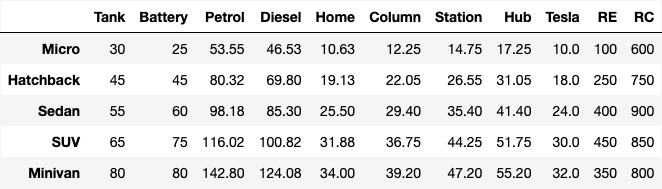
\includegraphics[width=\linewidth]{images/Prices_summary.png}
		\caption{Representative Fuel and Range Data for Cost Modeling}
		\label{fig: vehic_data}
		\captionsetup{font={footnotesize,bf,it}}
		\caption*{Data: ChatGPT (Estimates)}
	\end{center}	
\end{figure}
To assess the cost-efficiency of different vehicle types, a simplified metric was used by dividing the estimated driving range by the corresponding fuel or electricity price. This results in a “distance per euro” value, which reflects how many kilometers a vehicle can travel per unit of currency spent on energy.  While not a conventional efficiency measure like energy consumption per kilometer, it provides a useful comparison of economic driving performance across vehicle types and energy sources. This cost-based driving efficiency highlights the financial advantage of electric vehicles in scenarios with lower electricity prices and high energy efficiency
\begin{figure}[H]
	\begin{center}
		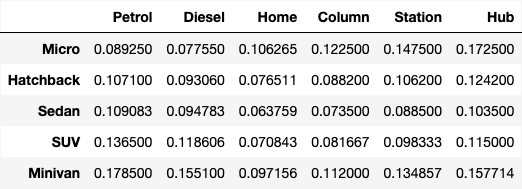
\includegraphics[width=\linewidth]{images/cost_efficiency.png}
		\caption{Cost Efficiency}
		\label{fig: Driving Efficiency}
		\captionsetup{font={footnotesize,bf,it}}
		\caption*{Data: ChatGPT (Estimates)}
	\end{center}	
\end{figure}
The cost per kilometer is consistently lower for electric vehicles compared to petrol and diesel across non-micro body types, especially when charged at home. Larger vehicles like SUVs and minivans show a more significant cost advantage when using home or standard charging options, highlighting the economic benefit of EVs in higher consumption segments. This analysis has focused on one aspect of a car's cost—charging expenses. However, a complete evaluation of a vehicle’s total cost of ownership also includes factors like resale value and operational costs.